% !TEX encoding = UTF-8
% !TEX TS-program = pdflatex
% !TEX root = ../tesi.tex
% !TEX spellcheck = it-IT

%**************************************************************
\chapter{Il contesto aziendale}
\label{cap:contesto-aziendale}
%**************************************************************

%\noindent Esempio di citazione in linea \\
%\cite{site:mediana}. \\

%\noindent Esempio di citazione nel pie' di pagina \\
%citazione\footcite{site:mediana} \\


%\begin{description}
%    \item[{\hyperref[cap:processi-metodologie]{Il secondo capitolo}}] descrive ...
    
%    \item[{\hyperref[cap:descrizione-stage]{Il terzo capitolo}}] approfondisce ...
    
%    \item[{\hyperref[cap:analisi-requisiti]{Il quarto capitolo}}] approfondisce ...
    
%    \item[{\hyperref[cap:progettazione-codifica]{Il quinto capitolo}}] approfondisce ..
    
%    \item[{\hyperref[cap:verifica-validazione]{Il sesto capitolo}}] approfondisce ...
    
%    \item[{\hyperref[cap:conclusioni]{Nel settimo capitolo}}] descrive ...
%\end{description}

%**************************************************************
\section{L'azienda}
\label{azienda}

Mediana S.r.l.u.(logo nella \hyperref[logoMediana]{Figura 1.1}) è una realtà aziendale nata nel 1994 con sede a Padova. Fondata nel pieno del boom dell'\acrshort{it} e all'inizio della diffusione su larga scala della connessione Internet, Mediana S.r.l.u. vuole imporsi sin da subito nel nuovo mercato dello sviluppo software. Inizialmente legata prettamente alla \acrshort{sfa}, con la liberalizzazione del mercato dell'energia l'azienda ha saputo rinnovarsi specializzandosi in modo deciso in un settore che presenta peculiarità tecniche, legislative e burocratiche, sviluppando prodotti specifici legati alla fatturazione dell'energia elettrica e del gas. Sebbene questo settore costituisca ancora il \textit{business core} dell'azienda, con il passare del tempo Mediana S.r.l.u. sta ampliando i propri orizzonti. Da un lato infatti i prodotti tradizionali legati al mondo dell'energia si stanno arricchendo di valore grazie all'apporto di nuove conoscenze ed esperienza. Dall'altro la nuova frontiera è rappresentata dalle soluzioni destinate all'utente finale, ovvero sia lo sviluppo di applicativi di gestione del \textit{business}, sia la realizzazione di strumenti di analisi per creare valore nella \gls{customer experience}. Forte di un'esperienza ventennale su campo nazionale e internazionale, Mediana S.r.l.u. ha sviluppato competenze specifiche ed evolvendosi dalla semplice vendita del prodotto \textit{software} al ruolo di \gls{system integrator} ha potuto garantire continuità nel rapporto con i propri clienti focalizzando il lavoro del proprio \textit{team} su un servizio di consulenza personalizzato.

\begin{figure}[ht]
\begin{center}

\includegraphics[height=50pt]{mediana_logo}
\caption{Logo Mediana S.r.l.u.}
\label{logoMediana}
\end{center}
\end{figure}

%**************************************************************
\clearpage
\section{Organizzazione aziendale}
\label{organizzazione}

L'azienda si compone di figure con competenze di tipo tecniche e amministrative diverse che possono assumere i seguenti ruoli:
\begin{itemize}
	\item\textbf{Project Manager}: gestisce le risorse e gli eventi del progetto. Essendo il punto di riferimento per l'intero progetto, è responsabile di tempi, costi e qualità del risultato finale. Si occupa infine di gestire eventuali \acrshort{cr} e fraintendimenti sulle specifiche di progetto;
	\item\textbf{Consulente business}: individua ambito ed obiettivi di progetto, verifica la sua fattibilità e tramite incontri di \textit{business} analisi con il cliente formalizza i requisiti. Deve essere poi in grado di far emergere le esigenze del cliente nell'ambito del progetto, al di là di quelle meramente espresse, in modo che la definizione del progetto che andrà a descrivere sia la più completa possibile;
	\item\textbf{Consulente tecnico}: crea il modello informatico della realtà di \textit{business}, verificando innanzitutto la fattibilità tecnica del progetto e facendo in seguito una stima dei tempi e delle risorse necessarie. Deve inoltre essere in grado di creare nuove configurazioni e inserire/modificare i dati degli utenti attraverso strumenti di manipolazione diretta dei dati come SQL. È necessario quindi che conosca le logiche di funzionamento delle applicazioni per le quali svolge questo ruolo;
	\item\textbf{Sviluppatore}: scrive \textit{software} nell'ambiente di sviluppo e nel \textit{database} scelto per l'applicazione seguendo le linee guida e gli standard definiti in azienda. Esegue inoltre i test di unità delle funzionalità che ha sviluppato;
	\item\textbf{Web designer}: realizza elaborati grafici di interfacce web, tablet, mobile che dovranno essere compatibili con la successiva implementazione da parte del \textit{team} di sviluppo. In continuo confronto sia con quest'ultimo che con il committente produce quindi dei \glspl{wireframe} per definire la struttura, gli elementi e il comportamento delle interfacce. Realizza infine dei \glspl{mockup} dettagliati che devono essere valutati e approvati dal committente e successivamente implementati dal \textit{team} di sviluppo. Offre inoltre supporto nella realizzazione di presentazioni volte alla promozione dei prodotti e servizi offerti dall'azienda.
\end{itemize}

Nella \hyperref[organigramma]{Figura 1.2} è possibile vedere una panoramica su come sono legati fra loro i ruoli appena descritti. Questi, a seconda delle esigenze, è probabile che vengano associati alla stessa persona, che quindi risulta avere diversi incarichi anche durante l'arco di vita dello stesso progetto.

\begin{figure}[ht]
\begin{center}
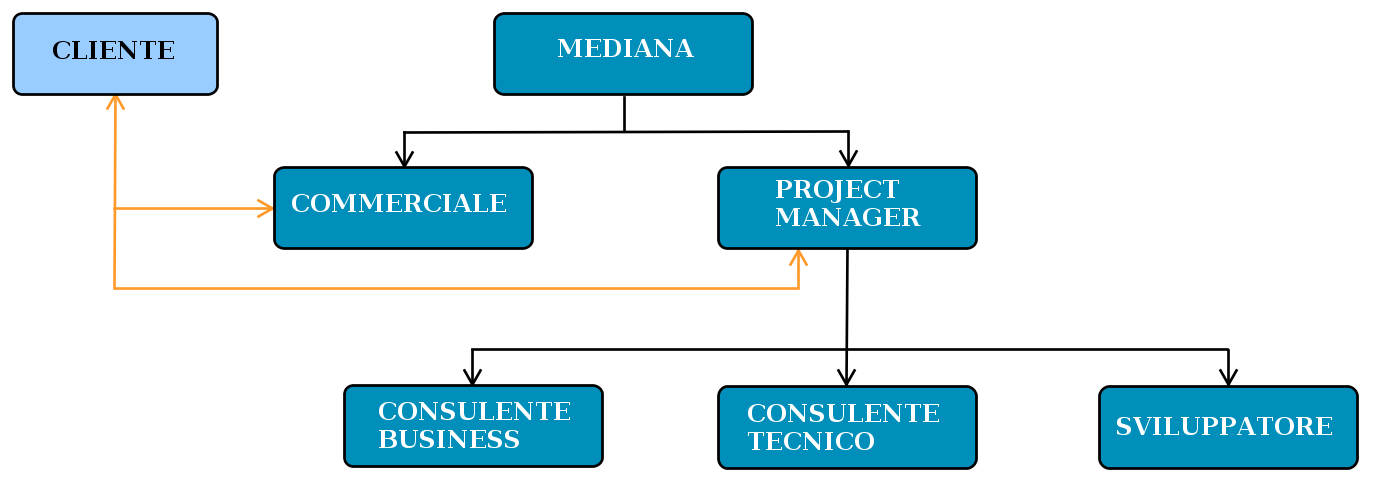
\includegraphics[scale=0.35]{OrganigrammaMediana}
\caption{Organizzazione per progetto in Mediana S.r.l.u.}
\label{organigramma}
\end{center}
\end{figure}
\FloatBarrier

%**************************************************************
\section{Prodotti aziendali}
\label{prodotti}

I prodotti di punta che l'azienda Mediana S.r.l.u. offre alla sua clientela sono:

\begin{itemize}
\item \textbf{XEnergy}: \textit{software} dedicato alle aziende che operano nel mondo dell'energia elettrica e gas, permette la gestione della fatturazione, dei preventivi, delle anagrafiche dei clienti e delle offerte, oltre che il controllo prezzo nella vendita sempre al passo con le novità di mercato e normative;
\item \textbf{XContract}: \textit{software} dedicato alla \acrshort{sfa}, permette l'inserimento e la gestione dei contratti per la vendita di energia elettrica e gas. Consente la corretta gestione del punto di fornitura, dall'inserimento a sistema all'attivazione del contratto, garantendo le tempistiche e il rispetto delle normative dell'Autorità garante per l'energia elettrica e gas;
\item \textbf{Web Portal}: \textit{software} che fornisce agli utenti delle aziende legate al mondo dell'energia elettrica e gas strumenti per monitorare lo stato delle loro fatture, consumi e contratti, sia tramite web che \textit{apps} \gls{ios} e \gls{android};
\item \textbf{CSIndex}: \textit{software} che consente di raccogliere il voto ed il feedback sia dei clienti di un'azienda che vende prodotti/servizi sia dei propri dipendenti (come descritto più approfonditamente nel \hyperref[cap:progetto-stage]{secondo capitolo}); permette poi di gestire le informazioni, visualizzare grafici ed estrazioni in base ai dati raccolti.
\end{itemize}

%**************************************************************
\section{Processi interni}
\label{processi}

In questa sezione descrivo il modello di ciclo di vita del \textit{software} utilizzato dall'azienda, le fasi che contraddistinguono un progetto dall'idea del cliente fino alla consegna del risultato finale. 

\subsection{Modello di ciclo di vita del software}
\label{ciclo di vita}
Nel fornire i progetti ex novo o effettuando cambiamenti evolutivi, Mediana S.r.l.u. segue un approccio incrementale che vede l'esecuzione delle fasi standard per macro \glspl{deliverable}. Viene quindi adottato un modello a spirale (rappresentato nella \hyperref[spirale]{Figura 1.3}) che abbraccia prototipazione, sviluppo iterativo del \textit{software}, e la valutazione del rischio. In questo modo lo sviluppo può essere arrestato alla fine di ogni ciclo a seconda della valutazione del ciclo precedente.

\begin{figure}[ht]
\begin{center}
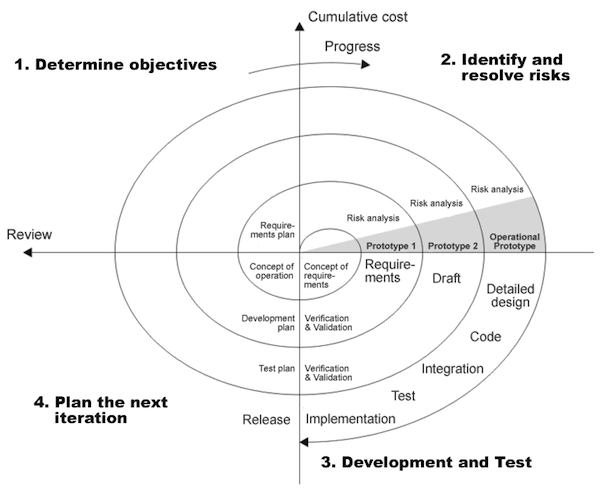
\includegraphics[scale=0.4]{ModelloSpirale}
\caption{Rappresentazione del modello di sviluppo a spirale}
\label{spirale}
\end{center}
\end{figure}
\FloatBarrier

\subsection{Le fasi di un progetto}
\label{fasi progetto}
Adesso vado ad analizzare le fasi che accompagnano la realizzazione di un progetto in Mediana S.r.l.u., specificando per ognuna di esse quali sono i documenti che le caratterizzano:

\begin{enumerate}
\item Una prima idea viene proposta al dipartimento \acrshort{it} dell'azienda cliente che redige un primo documento chiamato \textbf{Bill of Requirements} (\textbf{B.O.R.}) nel quale vengono riassunti i requisiti in modo molto generico;
\item Nella \textbf{Functional Analysis} (in caso di un nuovo prodotto) o \textbf{Gap Analysis} (nel caso di un'espansione di un prodotto già esistente) si analizza il \textbf{B.O.R.} per capire cosa si è in grado di realizzare e si fa quindi una prima stima di tempi e costi presentando una bozza delle possibili funzionalità che in futuro verranno sviluppate;
\item Si provvede poi a presentare un \textbf{documento di offerta} al cliente, contenente i costi e i tempi definitivi;
\item Approvata l'offerta viene creato un \textbf{diagramma di Gantt} al fine di pianificare, coordinare e tracciare le varie attività del progetto, che quindi viene ufficialmente lanciato (\textbf{Kick-off});
\item Mediana S.r.l.u. provvede quindi a redigere un documento, che dovrà essere confermato dal cliente, intitolato \textbf{Business Blue Print} (\textbf{B.B.P.}), nel quale vengono presentati i \glspl{mockup} e tutti i dettagli delle varie funzionalità che verranno poi implementate;
\item In seguito, con il cliente, si effettueranno regolarmente dei controlli per verificare che vengano rispettati i tempi come da pianificazione, riportando i dettagli nello \textbf{Stato di avanzamento dei lavori} (\textbf{S.A.L.});
\item Nella fase conclusiva del progetto vengono redatti gli \textbf{User Acceptance Test} (\textbf{U.A.T.}), con i quali Mediana S.r.l.u. conduce il cliente nell'effettuare, passo per passo, i test alle diverse funzionalità del \textit{software} in questione. In questo modo il cliente può verificare che l'applicativo funzioni correttamente;
\item In seguito, nel \textbf{Sir recap}, verranno segnalati tutti gli eventuali \textit{bug} da correggere o le \acrshort{cr} che sono sorte durante la fase di \textit{testing}. In base all'entità delle modifiche effettuate, o se ritenuto necessario, verranno ripetuti gli \textbf{U.A.T.};
\item Infine vengono redatti tutti i \textbf{manuali} necessari all'utente finale per comprendere al meglio il \textit{software} che dovrà utilizzare. Questi vengono consegnati al cliente durante la fase di prova del \textit{software} che da lì a breve verrà rilasciato in produzione.
\end{enumerate}

La \hyperref[fasiProgetto]{Figura 1.4} riassume tutte le fasi appena descritte, identificandole in base alla documentazione che le contraddistingue.

\begin{figure}[ht]
\begin{center}
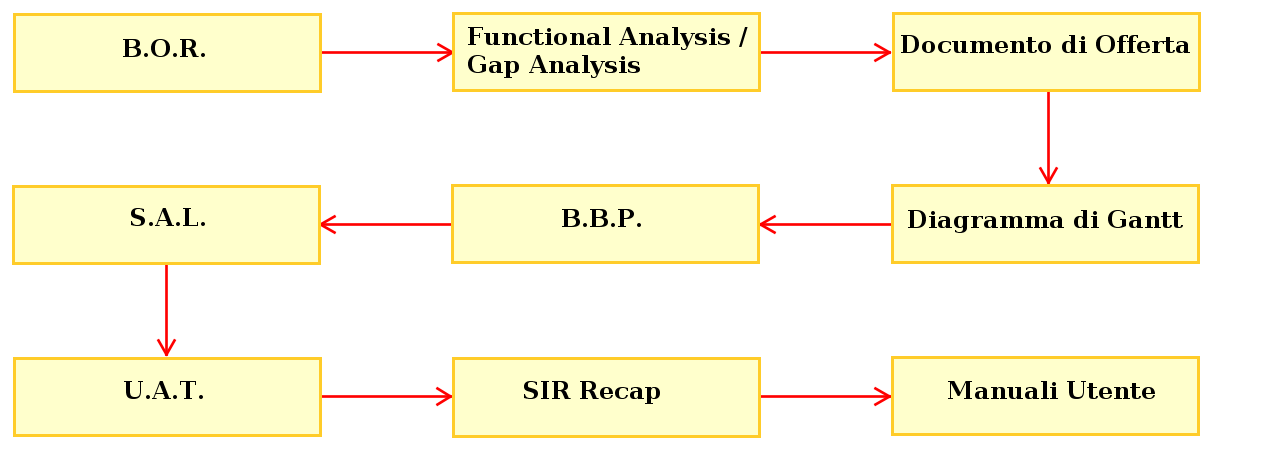
\includegraphics[scale=0.40]{FasiProgettoMediana}
\caption{Fasi di un progetto in Mediana S.r.l.u.}
\label{fasiProgetto}
\end{center}
\end{figure}
\FloatBarrier

\subsection{Ambienti di un programma}
\label{ambienti programma}
In base alla fase del progetto che si è raggiunta, il \textit{team} di Mediana S.r.l.u. rilascia i suoi \textit{software} nei seguenti ambienti così definiti:
\begin{itemize}
\item \textbf{Develoment environment (DEV)}: ambiente dove i programmatori creano le nuove applicazioni o aggiungono le nuove funzionalità richieste, tramite \acrshort{cr}, dal committente;
\item \textbf{Quality Assurance environment (QA)}: ambiente di test dove anche il committente può provare le funzionalità dell'applicativo concluso o aggiornato;
\item \textbf{Production environment (PROD)}: ambiente dove l'applicazione, che è stata approvata definitivamente dal committente, diventa fruibile all'utente finale.
\end{itemize}

\section{Strumenti e tecnologie a supporto dello sviluppo}
\label{strumenti e tecnologie}
Mediana S.r.l.u., nel sviluppare i propri \textit{software}, utilizza diversi strumenti e tecnologie.

\subsection{Sistemi operativi}
\label{sistemi operativi}
Il personale di Mediana S.r.l.u. utilizza per la maggior parte sistemi operativi \textbf{Windows}, salvo rari casi nei quali vengono utilizzati sistemi operativi \textbf{Mac OS} installati su macchine \textit{iMac} o \textit{MacBook Pro}.

\subsection{Tecnologie utilizzate}
\label{tecnologie}
Nella maggior parte dei progetti, Mediana S.r.l.u. utilizza le seguenti tecnologie:
\begin{itemize}
\item \textbf{ASP.NET}: insieme di tecnologie di sviluppo di \textit{software} per il web, commercializzate da \textit{Microsoft}. Sebbene il nome ASP.NET derivi da \acrshort{asp} (la vecchia tecnologia per lo sviluppo web di \textit{Microsoft}), esistono sostanziali differenze fra le due. Infatti ASP.NET si basa, come tutte le applicazioni della famiglia \textit{Microsoft} .NET, sul \acrshort{clr}. Le applicazioni ASP.NET sono significativamente più veloci e performanti rispetto a quelle realizzate utilizzando altre tecnologie di \textit{scripting}, in quanto l'intero codice del sito web è pre-compilato in pochi file \textit{dll} gestiti da un \textit{web server}. ASP.NET è progettato in modo da incoraggiare lo sviluppatore ad usare in modo sistematico il paradigma dell'interfaccia grafica abbinato alla cosiddetta programmazione ad eventi, cioè allo stile di programmazione in cui i vari blocchi di codice vengono eseguiti in risposta a determinati eventi su controlli dotati di rappresentazione grafica;
\item \textbf{HTML}: linguaggio di programmazione, e più nello specifico linguaggio di \textit{mark-up}, utilizzato per descrive il contenuto di una pagina web;
\item \textbf{CSS}: linguaggio usato per definire la formattazione delle pagine che costituisco un sito web, andando nello specifico a modificare il \textit{layout} di queste;
\item \textbf{Javascript}: linguaggio di \textit{scripting} orientato agli oggetti e agli eventi, comunemente utilizzato nella programmazione web lato \textit{client} per la creazione, in siti web e applicazioni web, di effetti dinamici interattivi. La caratteristica principale di JavaScript è quella di non essere un linguaggio compilato bensì interpretato. Viene utilizzato principalmente per scrivere piccole funzioni che vengono integrate nelle pagine HTML e che interagiscono con il \acrshort{dom} del browser per compiere determinate azioni non possibili con il solo HTML statico, come controllare i valori nei campi di ingresso, ecc.;
\item \textbf{C\#}: linguaggio di programmazione orientato agli oggetti sviluppato da \textit{Microsoft} all'interno dell'iniziativa .NET. La sintassi del C\# prende spunto da quella del Delphi (hanno il medesimo autore), del C++, di Java e anche in parte di Visual Basic per gli strumenti di programmazione visuale e per la sua semplicità;
\item \textbf{Transact-SQL}: versione proprietaria del linguaggio SQL sviluppata da \textit{Microsoft}, che ne estende le prestazioni aumentando:
\begin{itemize}
\item Funzioni per controllo di flusso;
\item Possibilità di definire variabili locali;
\item Varie funzioni per la manipolazione di stringhe ed altre tipologie di dati;
\item Possibilità di aggiungere, all'opzione \textit{FROM}, una \textit{JOIN} che permetta il collegamento tra più tabelle anche nelle operazioni di \textit{DELETE} e \textit{UPDATE}.
\end{itemize}
\end{itemize}

\subsection{Ambienti di sviluppo}
\label{ambienti sviluppo}
Gli \acrshort{ide} che vengono utilizzati per produrre il codice sono:
\begin{itemize}
\item \textbf{Microsoft Visual Studio}: ambiente sviluppato da \textit{Microsoft}, che supporta tutti i linguaggi legati al \textit{framework} .NET (compresi C\#, HTML e Javascript) e che permette la realizzazione di applicazioni, siti web, applicazioni web e servizi web.  Permette inoltre di correggere eventuali errori sintattici (ed alcuni logici) senza compilare l'applicativo, possiede poi un debugger interno per il rilevamento e la correzione degli errori logici nel codice in \textit{runtime} e fornisce diversi strumenti per l'analisi prestazionale;
\item \textbf{Microsoft SQL Server Management Studio}: ambiente pensato per l'accesso, la configurazione, la gestione, l'amministrazione e lo sviluppo di tutti i componenti di \textit{Microsoft SQL Server}. SQL Server Management Studio integra un'ampia gamma di strumenti grafici e editor di script avanzati per eseguire operazioni all'interno di \textit{database}. Tramite il cosiddetto \textit{Object Explorer} è poi possibile navigare, selezionare, e modificare tutti gli oggetti presenti all'interno dell'istanza di \textit{Microsoft SQL Server} (come per esempio \textit{database}, tabelle, ecc.).
\end{itemize}

\subsection{Software di versionamento}
\label{sw verionamento}
Vista la sua facile integrazione con il \textit{tool} di sviluppo \textit{Visual Studio}, Mediana S.r.l.u. ha deciso di adottare come \textit{software} per la gestione delle versioni dei suoi programmi \textbf{Microsoft Visual Sourcesafe}. Questo prodotto viene utilizzato per il controllo delle versioni a livello di \textit{file}, ciò consente al \textit{team} di utilizzare più versioni di un progetto contemporaneamente in modo da gestire versioni di codice parallele. Le funzionalità principali che Visual SourceSafe offre sono:
\begin{itemize}
\item Protezione del \textit{team} dalle perdite accidentali di \textit{file};
\item Controllo delle versioni precedenti di un \textit{file};
\item Supporto della diramazione, della condivisione, dell'unione e della gestione di versioni di \textit{file};
\item Controllo delle versioni di interi progetti;
\item Controllo di codice modulare (un \textit{file} riutilizzato, o condiviso, in più progetti).
\end{itemize}

\subsection{Software per la documentazione}
\label{sw documentazione}
Per la stesura di tutta le documentazione interna, ma anche per quella condivisa con i clienti e per quella destinata all'utente finale (come possono essere per esempio i manuali utente), Mediana S.r.l.u. utilizza \textbf{Microsoft Word}; uno dei programmi del suo genere più diffusi al mondo.

\subsection{Applicativi di supporto alla comunicazione e aggiornamento del lavoro}
\label{sw comunicazione}
Per tutte le comunicazioni interne si utilizzano le \textbf{e-mail} aziendali che vengono fornite al momento dell'assunzione; mentre per avere un continuo aggiornamento sullo stato dei lavori vengono condivisi dei documenti o fogli di calcolo online tramite \textbf{Google Drive}, un potente servizio di condivisione dati che consente il lavoro concorrente su di uno stesso \textit{file}.